%\documentclass[10pt, twocolumn]{article}
\documentclass[twocolumn,showpacs,preprintnumbers,amsmath,amssymb,prl]{revtex4}
%\documentclass[11 pt,preprint,preprintnumbers,amsmath,amssymb, prd]{revtex4}

% Preamble adapted from Surjeet Rajendran

\usepackage{latexsym}
\usepackage{amssymb}
\usepackage{epsfig,amsmath,graphics}
\usepackage{epstopdf}
\usepackage{verbatim}
\usepackage{wasysym}
\usepackage{hyperref}
\usepackage{feynmp-auto} % feynman diagrams
%\usepackage{subfig}
\usepackage[utf8]{inputenc}
\usepackage{xpatch}
\usepackage{xcolor}
\hypersetup{
    colorlinks,
    linkcolor={red!80!black},
    citecolor={green!60!black},
    urlcolor={blue!60!black}
}
\usepackage{appendix}

\newcommand{\OO}{\mathcal{O}}
\newcommand{\LL}{\mathcal{L}}
\newcommand{\HH}{\mathcal{H}}

\newcommand{\GeV}{\text{GeV}}
\newcommand{\MeV}{\text{MeV}}
\newcommand{\keV}{\text{keV}}
\newcommand{\rad}{\text{rad}}
\newcommand{\cm}{\text{cm}}
\newcommand{\angstrom}{\buildrel _{\circ} \over {\mathrm{A}}}
\newcommand{\pslash}{p\hspace{-0.070in}/\,}
\newcommand{\Mpl}{M_{\text{pl}}}
\newcommand{\ket}[1]{\ensuremath{\left|#1\right>}}
\newcommand{\bra}[1]{\ensuremath{\left<#1\right|}}
\newcommand{\braket}[2]{\ensuremath{\left<#1|#2\right>}}
%Large Parentheses
\def\r{\right)}
\def\l{\left(}

\begin{document}

\title{White Dwarves as Dark Matter Detectors}


\author{Ryan Janish}
\affiliation{Berkeley Center for Theoretical Physics, Department of Physics,
University of California, Berkeley, CA 94720, USA}

\author{Vijay Narayan}
\affiliation{Berkeley Center for Theoretical Physics, Department of Physics,
University of California, Berkeley, CA 94720, USA}

\author{Paul Riggins}
\affiliation{Berkeley Center for Theoretical Physics, Department of Physics,
University of California, Berkeley, CA 94720, USA}

\begin{abstract}

White dwarves can serve as detectors for ultra-heavy dark matter states which interact to trigger type 1A supernovae. This was originally proposed in \cite{Graham:2015apa} and used to place bounds on primordial black holes. In this paper we extend the capability of white dwarf detectors to candidates with non-gravitational couplings, focusing on dark matter transits and annihilations within the white dwarf. A benchmark model of this type is the baryonic Q ball in supersymmetric extensions of the standard model, which we are able to constrain well beyond current limits. More generally, we provide a detailed analysis of the explosiveness for any heating mechanism in the white dwarf initiated by strong or electromagnetic interactions. In this manner, white dwarves could constrain a variety of dark matter candidates including models of composite dark matter and self-interacting dark matter.  

\end{abstract}
\maketitle


\section{Introduction}

The detection of ultra-heavy dark matter (DM) is an open problem which will ultimately require a confluence of astrophysical probes. \textcolor{red}{Comment on the fundamental limit of terrestrial detectors at high masses?} One such proposal originally introduced by \cite{Graham:2015apa} is the possibility for DM to trigger supernovae in sub-Chandrasekhar white dwarves via localized heating and induced runaway fusion. 

In order to initiate runaway fusion in a star, a region must be sufficiently heated to the point where fusion reactions occur.  Each fusion reaction releases additional energy that heats neighboring regions until they can support fusion as well. In this manner the fusing volume increases until enough energy has been released to destroy the star.  However, the fusion region is also simultaneously cooling by a variety of mechanisms - if any of these processes drain energy from the region faster than it is liberated by fusion, there will be a quench of the nascent fusion chain-reaction. In a white dwarf (WD) there are fewer cooling mechanisms than in a non-degenerate star. Namely, WD cooling must rely on thermal diffusion whereas main-sequence stars can also cool via thermal expansion. Fundamentally this is due to the fact that a WD is supported against collapse by electron degeneracy pressure, which is independent of temperature. 

For a carbon-oxygen WD, the \emph{fusion temperature} $T_F$ is the onset temperature of carbon-carbon fusion. This is set by the energy required for carbon ions in the star to overcome their mutual Coulomb barriers, and is thus a constant $T_F \sim \MeV$. WD cooling is set by the thermal diffusivity of photons and degenerate electrons. The two species dominate the cooling at different stellar densities, as determined precisely by \cite{Woosley}. Notably, for a heated region of size $R$ this cooling rate $\propto R^2$ while the fusion rate $\propto R^3$. Thus, there is a critical \emph{trigger size} $\lambda_T$ below which diffusive cooling dominates the thermal evolution of a temperature peak, and above which the liberated fusion energy dominates \cite{Woosley}. Note that $\lambda_T$ (as defined) is highly sensitive to the WD density and has been analytically scaled for varying WD masses in \cite{Graham:2015apa}. These results are reproduced in Figure~\ref{fig:triggersize}. As in \cite{Graham:2015apa}, we restrict our attention to carbon-oxygen WDs in the upper mass range $0.7 - 1.4 ~M_{\odot}$ which correspond to a number density of nuclei $n \sim 10^{29} - 10^{32} ~\cm^{-3}$. Over this range, the trigger size is approximately $\lambda_T \sim 10^{-5} - 10^{-2} ~\text{cm}$. 

Therefore, a region with temperature greater than $T_F$ and size greater than $\lambda_T$ in a given WD will launch a runaway fusion chain-reaction and result in a type IA supernovae. If any process involving DM is able to achieve these conditions, white dwarves are uniquely qualified to either confirm such a model or, most likely, place novel constraints. In this regard, white dwarves can serve as detectors for ultra-heavy DM states which interact to trigger supernovae. This was initially implemented by \cite{Graham:2015apa} in order to constrain primordial black holes which would ignite the star through gravitational heating. In this paper, we extend the analysis of \cite{Graham:2015apa} to DM candidates with generic non-gravitational couplings, focusing on DM transits and annihilations within the WD which release energy in the form of standard model (SM) particles. A benchmark model of this type is the baryonic Q ball in supersymmetric extensions of the SM, which we are able to constrain many orders of magnitude beyond current terrestrial-based limits. More generally, we provide a detailed analysis of the explosive power of any heating mechanism in the white dwarf initiated by strong or electromagnetic interactions.  


\textcolor{blue}{Weaknesses - other ignition sources exist (i.e., detector backgrounds). What constraints can be placed in light of this?}


\section{Overview}

A general energy deposition event in the WD can be roughly characterized by two parameters: a temperature $T$ and heating length $L$. This energy deposit will eventually take the form of a local peak in the WD temperature profile. We define $T$ to be the characteristic temperature and $L$ the characteristic length scale of this local peak as it initially appears.  

$L$ is determined by the efficiency with which a given energy deposition mechanism interacts with the stellar medium. For instance, suppose that kinetic energy were transferred directly to neighboring ions via elastic scatters. These ions would thermalize over their collisional time scale resulting in a heating length $L$ of order the ion mean free path. In fact, this is the minimal $L$ possible for any process which couples to WD constituents (ions or electrons). \textcolor{red}{If we want to use this example, let's check it carefully by doing the calculation (VJ).} \textcolor{blue}{In the other extreme, suppose that a process produces a large number of electrons with energy just above the Fermi energy.  These electrons have Pauli-suppressed interactions with the medium and will travel a long distance before their energy is scattered and thermalized, resulting in a large $L$ - possibly of order the stellar radius.}  

In this paper, we focus on (nonelastic) DM interactions which heat the star via the production of high-energy standard model particles. Understanding the heating lengths of these processes is critical to assessing their explosive potential - these heating lengths are presented in section~\ref{sec:heatinglengthsummary} and computed in detail in appendix~\ref{app:heatinglengthfull}.  In our processes, typical $L$ will range from $10^{-7} \cm$ to $0.1 \cm$.

We need a condition that determines if a given heating event $L$, $T$ will result in the destruction of the star as a supernova.  It will be more useful to phrase this in terms of the excess energy $E$ within the temperature peak instead of the temperature itself $E \sim n T L^3$. The explosion condition is then:
\begin{equation}
\label{eqn:boom}
E_{\text{boom}} \gtrsim n T_B \text{Max}\left[L, \lambda_T\right]^3. 
\end{equation}
Note that this condition determine if a region $L$, $T$ \emph{immediately} initiates runaway fusion.  But what we are concerned with in this work is whether a given energy deposit \emph{eventually} initiates runaway fusion.  If $T < T_B$, then fusion will never occur. But, if $T >> T_B$ with $L < \lambda_T$, then while the thermal evolution is initially dominated by diffusive cooling it is possible that it evolves into a temperature profile with $L > \lambda_T$ while still having $T > T_B$. At that point, runaway fusion will begin.  Since diffusion dominates while $L<\lambda_T$, the thermal evolution will to lowest order be given by the dilution of the fixed total energy of the initial region over the final volume.  The temperature of the peak when it has diffused out to a size $\lambda_T$ is thus:
\[
    T_{\text{after diffusion}} \sim T \l \frac{L}{\lambda_T} \r^3  
\]
For this to be above the fusion onset temperature, we have the condition on the initial temperate and size:
\[
    T \gtrsim T_B \l \frac{\lambda_T}{L} \r^3
\]
which applies specifically to the case $L < \lambda_T$. Thus to eventually initiate fusion from a region smaller than the trigger size, one needs to begin with a temperature parametrically larger than $T_B$.  Combining this with the fusion condition for $L>\lambda_T$, we have the full condition to eventually ignite runaway fusion:
\[
    T \gtrsim T_F \text{Max}\left[1, \frac{\lambda_T}{L}\right]^3
\]
 This is just condition~\ref{eqn:boom}, after replacing the peak temperature $T$ for the total initial energy.


The moral of condition~\ref{eqn:boom} is that to destroy a white dwarf one needs to deposit both enough energy and enough energy density.  There is an absolute minimum explosion energy:
\[
    E_{\text{min}} \sim n T_B \lambda_T \sim 10^{\text{\textcolor{blue}{something}}} - 10^{14} \GeV
\]
(the range here is due to the range in white dwarf densities).  Yet this energy is sufficient only if it thermalizes below the trigger size.  If your energy is deposited on a length scale larger than $\lambda_T$, the explosion energy required is parametrically larger. As we are concerned with processes that have a fixed deliverable energy (the energy of the incoming DM), the most explosive processes will be those that result in the most localized heating.

\begin{figure}
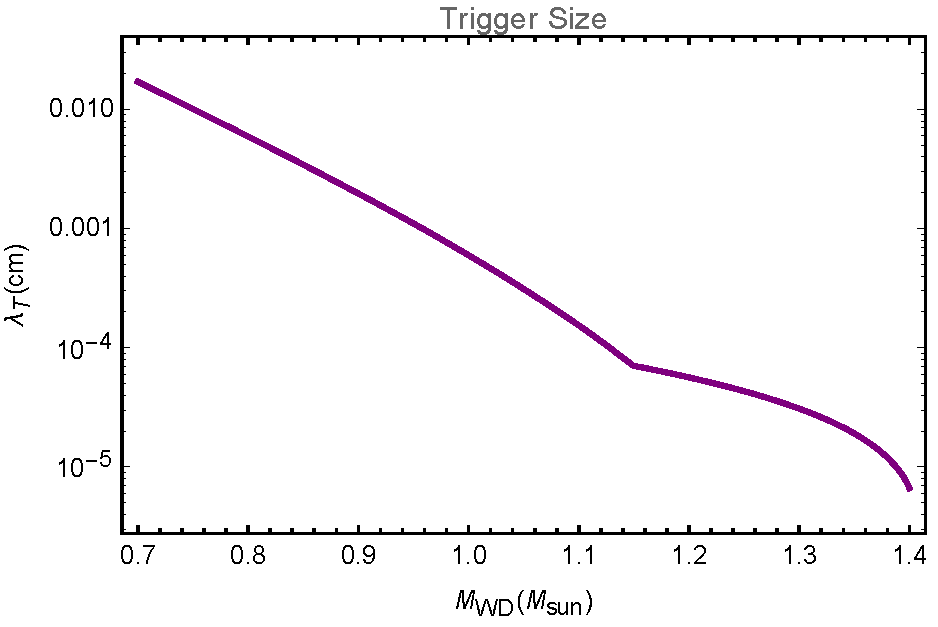
\includegraphics[scale=.45]{triggerboom.pdf}
\caption{Approximate trigger sizes for carbon-oxygen white dwarfs, as calculated in~\cite{Graham:2015apa}.
\textcolor{blue}{extend this to smaller masses - 0.4 is minimum wd mass}}
\label{fig:triggersize}
\end{figure}

\section{DM Explosivness}
In this section, we parameterize the potential explosiveness of DM interactions in the WD. 

\subsection{DM Transit through the WD}

\subsection{DM Annihilation in the WD}

Consider an ultra-heavy dark matter (DM) state transit through the WD. Assume that the DM interacts with WD constituents (ions or electrons) in a general manner as shown in Figure \ref{fig:feynmandiag}, releasing $n_i$ particles of species $i$ each with kinetic energy $\epsilon$. The cross section for this interaction is denoted as $\sigma_{i,\epsilon}$. Of course, this released energy must be transferred to the stellar medium in order for the WD to be heated. For a given particle type, each value of $\epsilon$ is characterized by a distance $R_\epsilon$ from the point of release over which it is deposited. This thermalization distance is the nominal size of any resulting hot region and is set by the various ways in which emitted particles interact with stellar constituents. In particular, we define $R_\epsilon$ as the distance over which a particle $i$ and any secondaries transfer $\OO(1)$ of the initial energy $\epsilon$ to electrons or ions in the WD. To demonstrate the significance of this parameter, suppose that the DM simply scattered off nuclei elastically with no particles released. In this case, $R_\epsilon$ effectively vanishes as $\epsilon$ is transferred directly to the kinetic energy of nuclei. However, in the other extreme limit, suppose the interaction released energy into neutrinos. In this case, $R_\epsilon$ is of astronomical length scales and there would be no chance of thermalizing any local region in the star. 

\begin{figure}
\label{fig:feynmandiag}
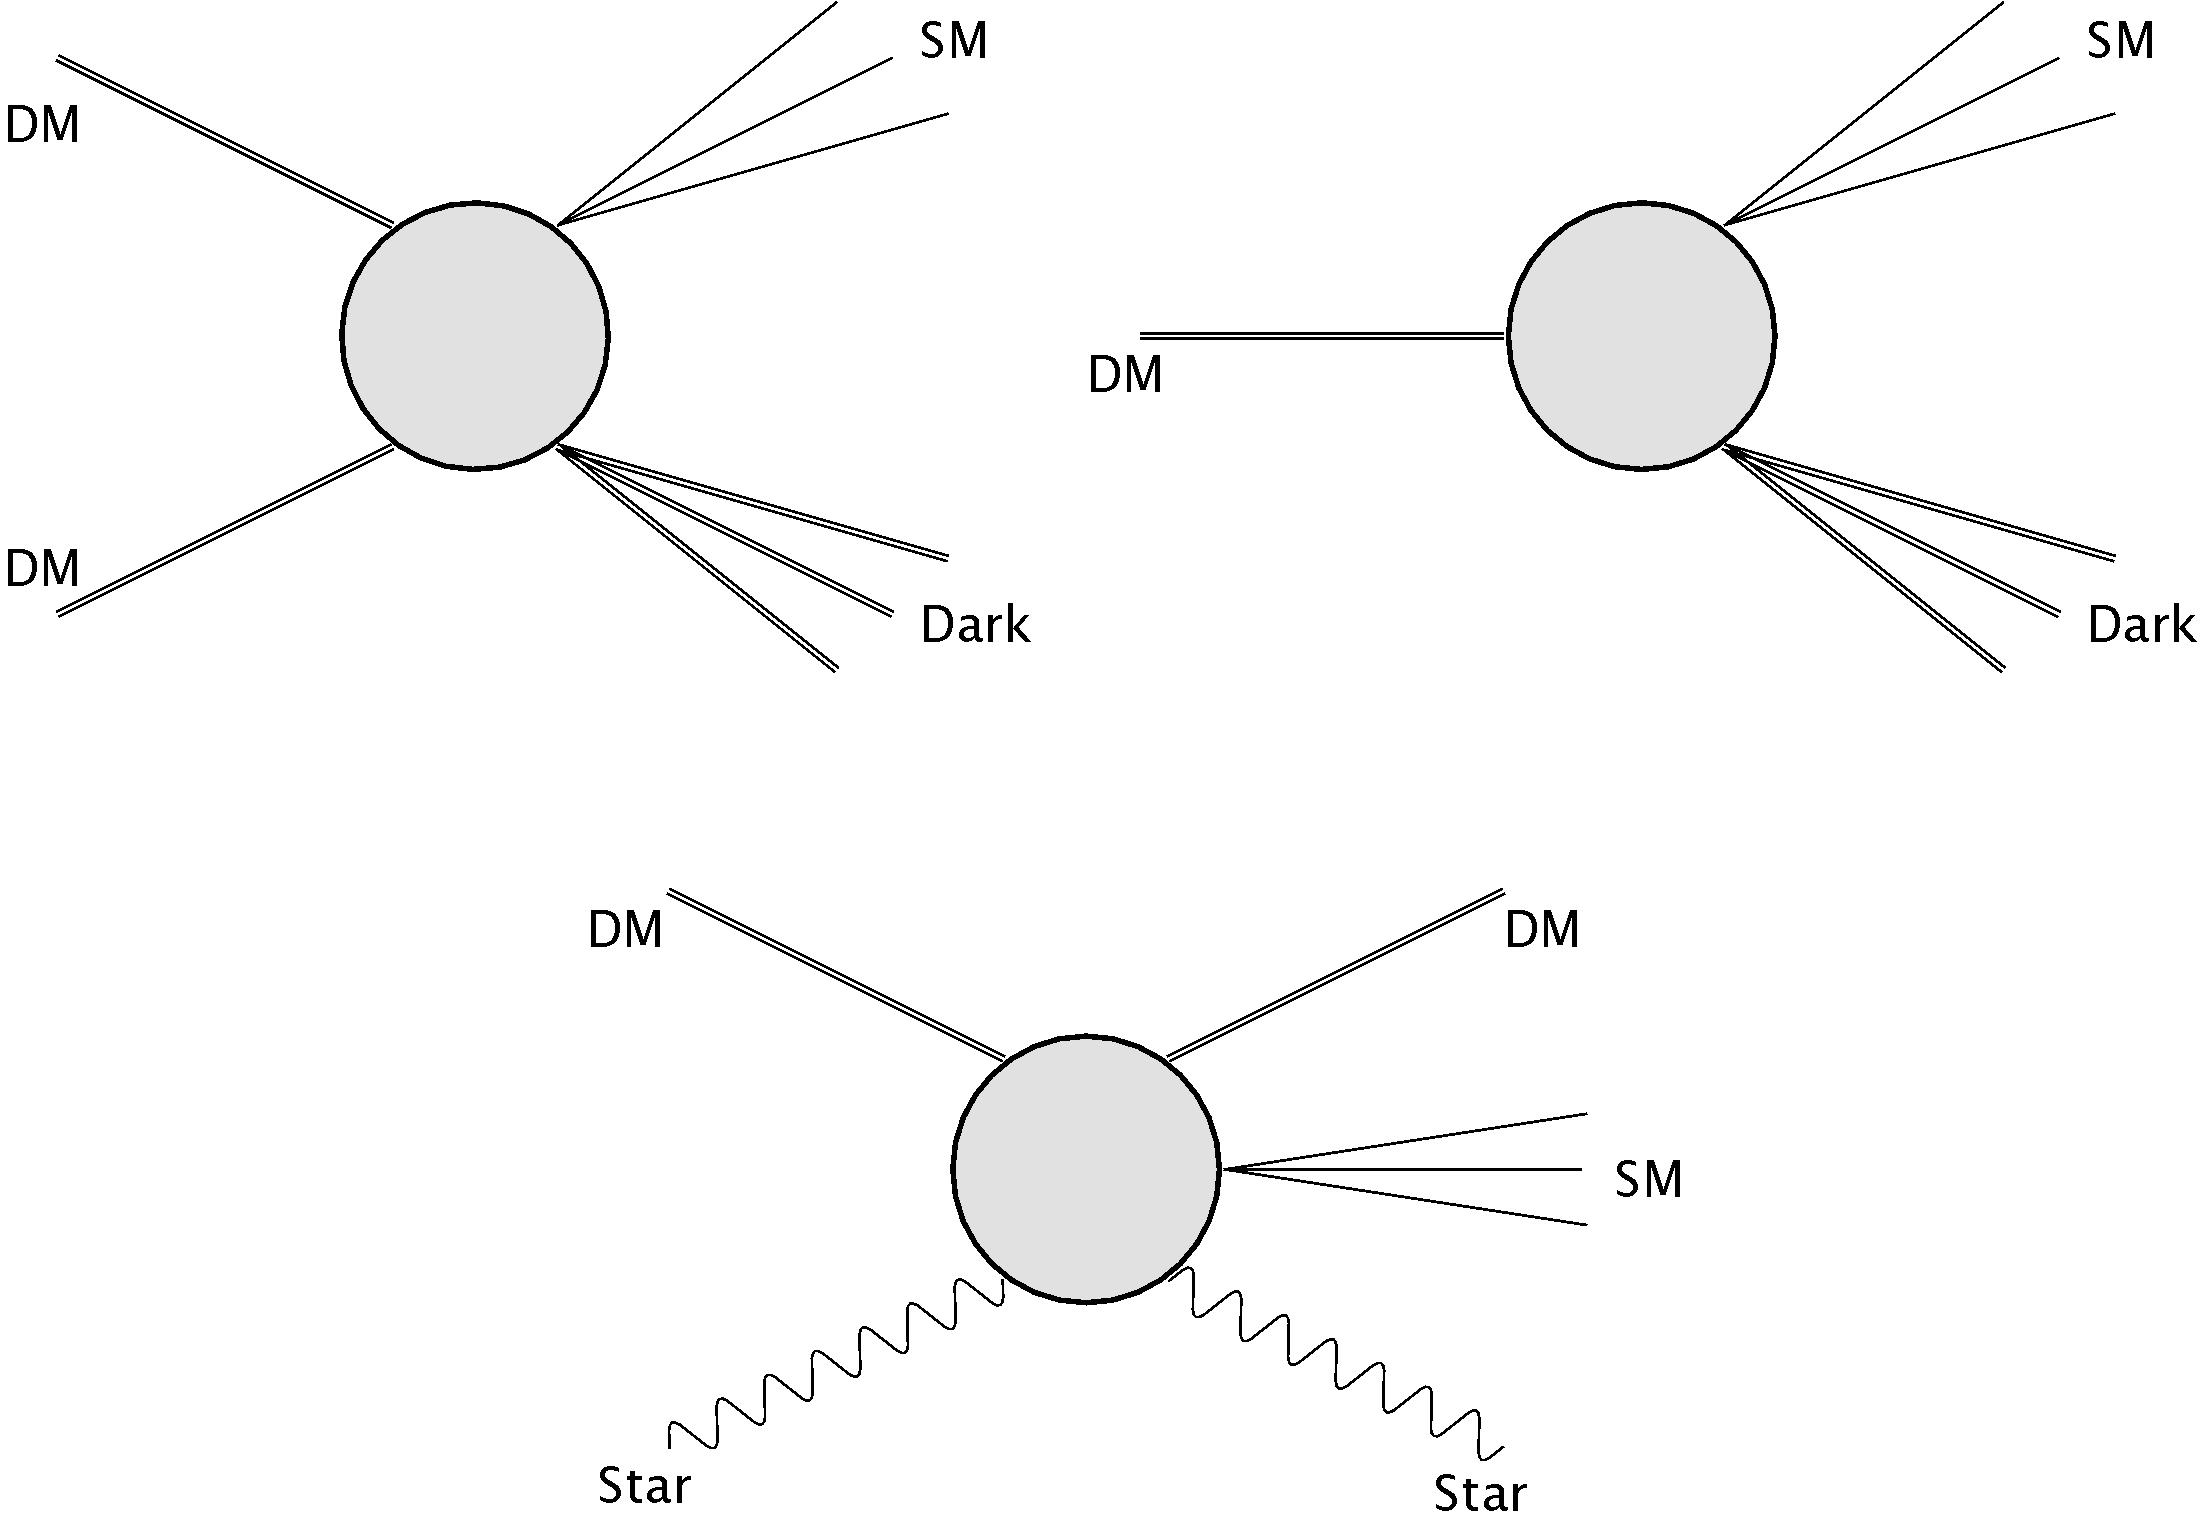
\includegraphics[scale=.05]{feynmandiag}
\caption{General interaction between ultra-heavy DM and WD constituents, producing $n_i$ additional particles of species $i$.}
\end{figure}

Consider the two possibilities relevant for ignition. If $R_\epsilon> \lambda_T$, the DM must deposit a minimum energy $E_{\text{boom}} \sim R_\epsilon^3 n T_f$ in order to heat up the entire region of size $R_\epsilon$ to the critical temperature $T_f$, where $n$ is the number density of nuclei in the WD. On the other hand, if $R_\epsilon < \lambda_T$ then the minimum energy required is independent of $R_\epsilon$ and given by $E_{\text{boom}} \sim \lambda_T^3 n T_f$. Setting $T_f \sim \text{MeV}$, $\lambda_T \sim 10^{-5} ~\text{cm}$, and $n \sim 10^{32} ~\text{cm}^{-3}$, we find that an energy $E_{\text{boom}} \sim 10^{14} ~\text{GeV}$ transferred to the WD within a localized region smaller than $\lambda_T^3$ will eventually trigger runaway fusion. This ``explosion" energy must be less than the total energy released during the DM transit. Doing so, we find a lower bound on the interaction cross section sufficient to trigger runaway fusion: 

\begin{equation}
\label{eq:explosion}
n_i \sigma_{\epsilon,i} \gtrsim \left\{
        \begin{array}{ll}
            \displaystyle \lambda_T^2 \l \frac{T_f}{\epsilon} \r & \quad R_\epsilon < \lambda_T \\
             \lambda_T^2 \l \frac{R_\epsilon}{\lambda_T}\r^2 \l \frac{T_f}{\epsilon} \r & \quad R_\epsilon > \lambda_T
        \end{array}
    \right..
\end{equation}

Note that in deriving this explosiveness bound, we have assumed the DM transit time is less than the corresponding diffusion time. After a time $\Delta t$ the DM has traversed $v_{\text{esc}} \Delta t$, where the velocity is set by the escape velocity of a WD. Therefore, this amounts to the following condition:
\begin{equation}
\begin{array}{ll}
             \tau_d(\lambda_T, T_f) \gtrsim \frac{\lambda_T}{v_{\text{esc}}}, & \quad \quad R_\epsilon < \lambda_T \\ \\
            \tau_d(R_\epsilon, T_f)  \gtrsim \frac{R_\epsilon}{v_{\text{esc}}},  & \quad \quad R_\epsilon > \lambda_T
        \end{array}
\end{equation}
where $\tau_d$ is the characteristic time for a region of given size and temperature to diffuse $\OO(1)$ of its heat. An estimate from the heat equation gives $\tau_d(\lambda_T, T_f) \sim \frac{\lambda_T^2}{\alpha}$, where $\alpha$ is the (temperature-dependent) diffusivity. \textcolor{blue}{Show condition is true for all densities.} We also assume that the time to transfer energy $\epsilon$ out to its characteristic range $R_\epsilon$ is less than the diffusion time scale $\tau_d(\lambda_T, T_f)$.

\section{General Constraints}

\subsection{Annihilation Events: Rate and Constraints}

\subsection{Transit Events: Rate and Constraints}

\section{Heating Lengths}
\label{sec:heatinglengthsummary}

<<<<<<< Updated upstream
In this section, we enumerate the different ways in which standard model particles can lose energy to the WD. (Unless otherwise noted, we will assume a carbon-oxygen white dwarf.) The interior of a WD is a complex environment. Famously, the star is supported against collapse by electron degeneracy pressure with a characteristic Fermi energy $E_F \sim n_e^{1/3} \sim \OO(\text{MeV})$ \textcolor{red}{at all densities?}. In addition, the nuclei are at an ambient temperature $T \sim \text{keV}$ and form a strongly-coupled plasma $\frac{Z e^2}{n^{1/3} T} \gg 1$. In what follows, we calculate the WD medium sensitivity to deposited energy and the deposit ranges $R_\epsilon$ for the different possible DM interactions. For the purpose of depositing sufficient energy to trigger supernovae, we focus on high-energy particles $\epsilon \gg \text{MeV}$ which interact via the strong and electromagnetic forces (i.e. electrons, muons, photons, pions, and neutral hadrons). In this way, the WD may be thought of as a ``particle detector" with electromagnetic and hadronic ``calorimeter" components.
=======
In this section, we enumerate the different ways in which standard model particles can lose energy to the WD. The interior of a (carbon-oxygen) WD is a complex environment. Famously, the star is supported against collapse by the degeneracy pressure of an electron gas at a characteristic Fermi energy $E_F \sim n_e^{1/3} \sim \OO(\text{MeV})$. In addition, the nuclei are at an ambient temperature $T \sim \text{keV}$ and form a strongly-coupled plasma $\frac{Z e^2}{n^{1/3} T} \gg 1$. In what follows, we calculate the WD medium sensitivity to deposited energy and, in turn, $R_\epsilon$ for the different possible DM interactions. For the purpose of depositing sufficient energy to trigger supernovae, we focus on high-energy particles $\epsilon \gg \text{MeV}$ which interact via the strong and electromagnetic forces (i.e. electrons, muons, photons, pions, and neutral hadrons). In this sense, the WD may be thought of as a ``particle detector" with electromagnetic and hadronic ``calorimeter" components.  
>>>>>>> Stashed changes

\subsection{Electromagnetic Interactions}

For charged particles, Coulomb scattering is a useful mechanism for energy transfer. Generically, an incident (spin-0) particle of mass $m_i$, charge $e$, and velocity $\beta$ scattering off a target $M_t$ of charge $Ze$ is described by the ``Rutherford" differential cross section \textcolor{blue}{Originally derived by Bhabha?}
\begin{equation}
\label{eq:rutherford}
\frac{d \sigma}{dE'} = \frac{2 \pi  \alpha^2 Z^2}{M_t \beta^2} \frac{1}{E'^2} \l1- \frac{\beta^2 E'}{E_{\text{kin}}}\r,
 \end{equation}
where we have assumed a sufficiently fast incident particle so that interactions are governed by single collisions with energy transfer $E'$ \cite{Agashe:2014kda}. $E_{\text{kin}}$ denotes the maximum energy transfer possible satisfying kinematic constraints \textcolor{blue}{target at rest and zero relative angle between incoming incident and outgoing target momenta}:
\begin{equation}
E_{\text{kin}} = \frac{2 M_t \beta^2 \gamma^2}{1+ 2\gamma(M_t/m_i) +(M_t/m_i)^2},
\end{equation}
where $\gamma = (1-\beta)^{-1/2}$.

For sufficiently heavy incident particles, the differential cross section depends only on the velocity of the incident particle. Note that higher-spin particles receive additional corrections to the cross section, but for small energy transfers these corrections are negligible. It is straightforward to understand the parametric dependences of \eqref{eq:rutherford}: there is increased likelihood to scatter for slowly moving incident particles undergoing ``soft-scatters" against lighter targets. Therefore, one would expect that soft scattering dominates the energy loss and that collisions with nuclei of mass $M$ are suppressed by a factor $\OO\l\frac{Z m_e}{M}\r$ as compared to collisions with electrons. This is certainly true for incident charged particles in non-degenerate matter. However, both of these naive expectations turn out to be false when considering scattering off a degenerate species.

To understand the effect of degeneracy, we first consider the energy loss from scattering a high-energy charged particles off non-degenerate targets in the WD, for instance, the carbon nuclei. In this case, the stopping power due to collisions with a number density $n$ is given by:
\begin{align}
\label{eq:SP}
\frac{dE}{dx} & = - \int dE' \left(\frac{d \sigma}{dE'}\right) n E' \\
& \sim -\frac{2 \pi n Z^2 \alpha^2}{M_t \beta^2} \log{\l\frac{E_{\text{max}}}{E_{\text{min}}}\r}.
\end{align}
This integration must be performed over all $E'$ within the regime of validity for \eqref{eq:rutherford}, fixing the lower and upper bounds of the ``Coulomb Logarithm". Quantum mechanical uncertainty sets a limit to the accuracy that can be achieved in ``aiming" an incident particle at a target. In terms of impact parameter $b$ for the collision, this translates to a bound $b \gtrsim (\text{min}\{{m_i, M_t}\} \beta \gamma)^{-1}$ corresponding to the larger de Broglie wavelength. In terms of energy transfer, this becomes
\begin{equation}
E' \lesssim E_q = \frac{2 ~\text{min}\{{m_i, M_t}\}^2 Z^2 \alpha^2 \gamma^2}{M_t}.
\end{equation}
In addition, the expression for the differential cross section \eqref{eq:rutherford} no longer holds when $E'$ becomes larger than the mass of the target \cite{Rossi}. For our calculations, we take the maximum energy that an incident particle is able to transfer to be
\begin{equation}
E_{\text{max}} = \text{min}\{E_q, E_{\text{kin}}, M_t\}.
\end{equation}
On the other hand, the maximum impact parameter is determined by charge screening. In a WD, this is simply the screening due to a degenerate electron gas \textcolor{blue}{similar to a solid} and is given by the Thomas-Fermi length \cite{Teukolsky}
\begin{equation}
l_{\text{sc}} = \l\frac{6 \pi Z e^2 n_e}{E_F}\r^{-1/2}\sim \frac{1}{m_e}.
\end{equation}
\textcolor{blue}{This is the equivalent of the Debye screening length for a degenerate gas at Fermi energy $E_F$}. This corresponds to a lower bound
\begin{equation}
E_{\text{sc}} = \frac{2 m_e^2 Z^2 \alpha^2}{M_t \beta^2}.
\end{equation}
Note that when the incident particle reaches velocity $\beta \gamma \approx \frac{m_e}{\text{min}\{m_i, M_t\}}$, the minimum possible energy transfer due to Thomas-Fermi screening will in fact exceed the maximum. At this point, the form of equation \eqref{eq:SP} becomes modified to avoid unphysical non-negative values of $dE/dx$ and there is negligible stopping power due to collisions. However, the lattice structure of ions in the WD introduces further complications \cite{Teukolsky}. The typical lattice binding energy between ions is given by the electric potential
\begin{equation}
E_B \sim \frac{Z^2 e^2}{n^{-1/3}}.
\end{equation}
For energy transfers greater than $E_B$, any lattice effects can be safely ignored. On the other hand, momentum transfers from collisions below this threshold may lead to suppressed energy loss due to collective effects. For simplicity we set the lower bound on nuclei scattering (not applicable for electron targets) to be
\begin{equation}
E_{\text{min}} = \text{max} \{E_B,E_{\text{sc}}\}
\end{equation}
so that we only account for energy transfers greater than the ionic lattice binding energy.

When considering collisions with the degenerate electrons, an incident particle transferring energy $E'$ can only scatter those electrons within $E'$ of the Fermi surface. We define a modified density of electrons $n_e(E')$ as:
\begin{equation}
n_e(E') = \left\{
        \begin{array}{ll}
            \displaystyle \int \limits_{E_F -E'}^{E_F}dE ~g(E) & \quad E' \leq E_F \\
            n_e & \quad E_F \leq E'
        \end{array}
    \right.,
\end{equation}
where $g(E)$ is the density of states per unit volume for a three-dimensional free electron gas. This can also be expressed as a suppression of the differential cross section of order $\mathcal{O}(E'/E_F)$ whenever energy less than $E_F$ is transferred. Therefore, unlike in the non-degenerate case, the energy loss due to soft-scatters are in fact subdominant to the contributions from rare hard-scatters. The stopping power is also highly sensitive to $E_{\text{max}}$ and $E_{\text{min}}$, governed by a power-law dependence rather than the logarithmic sensitivity in the case of a non-degenerate target.

We have calculated the stopping power of high-energy particles solely due to Coulomb collisions, differentiating between nuclei and degenerate electron targets. This is shown in Figure \textcolor{blue}{figure} for an electron density $n_e \sim 10^{33} ~\text{cm}^{-3}$. It is found that for heavy incident particles, the stopping power is dominated by collisions with nuclei at low-energies although it is dominated by collisions with degenerate electrons at high-energies. In addition, scattering off degenerate electrons becomes completely screened at a comparatively higher energies.

\begin{figure}
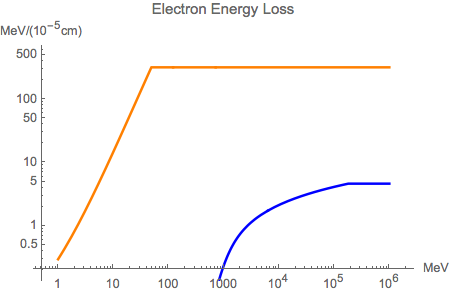
\includegraphics[scale=.4]{electronenergyloss}
\end{figure}

\begin{figure}
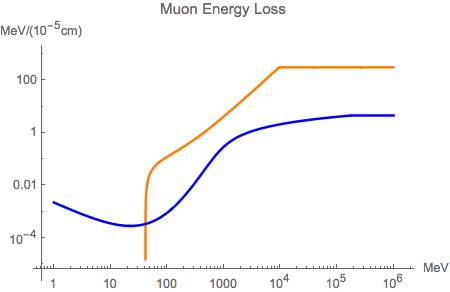
\includegraphics[scale=.4]{muonenergyloss}
\end{figure}

\begin{figure}
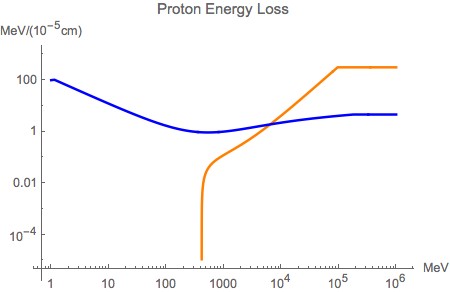
\includegraphics[scale=.4]{protonenergyloss}
\end{figure}

\subsection{Strong Interactions}

Strong interactions are a significant channel for energy transfer in the WD. For sufficiently energetic particles greater than the nuclear binding energy $E_{nuc} \sim \OO(10 ~\text{MeV})$, nuclear interactions (absorption) result in an $\OO(1)$ number of energetic secondary hadrons (protons, neutrons, pions, etc.) emitted roughly in the direction of the primary particle. These secondary particles approximately split the initial total energy of the absorbed primary particle and can collide with other nuclei in the WD. In addition, the nucleus will generally be left in an excited state and relax through the emission of low-energy $\OO(10 ~\text{MeV})$ nucleons (``nuclear evaporation") and photons \cite{Rossi}. The cross section for any such process is approximately set by the nuclear length scale $\sim \text{fm}$. A hadronic shower is a result of all such reactions caused by primary and secondary particles.

To estimate the typical shower length, we assume a primary particle of energy $\epsilon$ interacting with nuclei to produce $N$ secondary particles each of energy $\epsilon/N$. The shower will end once final-state particles reach energies of order $E_{nuc}$. We ignore the effects of the evaporative stage in each reaction as this will only introduce minor corrections at sufficiently large $\epsilon$. We find a hadronic shower length $L = l_\text{nuc} \l \frac{\log{(\epsilon/E_{nuc})}}{\log{N}}\r$, where $l_\text{nuc}$ is the mean free path for nuclear collisions. For a number density $n \sim 10^{32} ~\text{cm}^{-3}$ and hadronic cross section $\sim 0.1 ~\text{barn}$ \textcolor{blue}{match nuclear data for carbon nonelastic scattering} this results in a shower length $L \approx 10  ~l_\text{nuc} \approx 10^{-6} ~\text{cm}$. Note that this only has a mild, logarithmic sensitivity to the initial energy $\epsilon \gg ~\text{10 ~\text{MeV}}$ and number of secondaries $N \sim \OO(1)$.

The end products of a hadronic shower will generally be hadrons of kinetic energy $1-10 ~\text{MeV}$ which are incapable of inducing further nuclear disintegration. Charged hadrons have appreciable electromagnetic interactions with nuclei, while collisions with degenerate electrons are completely screened at these energies. Integrating \eqref{eq:SP}, we find that in a density of $n \sim 10^{32} ~\text{cm}^{-3}$ protons traverse $\approx 10^{-6} ~\text{cm}$ slowing down from 5 MeV to 1 MeV. \textcolor{blue}{The corresponding distance is significantly larger for charged pions $\sim 10^{-2} ~\text{cm}$} On the other hand, electromagnetic couplings are highly suppressed for final-state neutral hadrons. The dominant source of energy loss for neutrons in this range is elastic scattering off nuclei \textcolor{blue}{neutron capture cross section in C+O is negligible}. Each scatter transfers a fraction $\l1-\l\frac{m}{m + M}\r^2\r \approx 0.1$ of the neutron energy to nuclei (averaging over scattering angles), where $m$ and $M$ are the masses of the neutron and nuclei, respectively.  At kinetic energies below $\sim \text{MeV}$, the typical energy transfer in an elastic collision is of order the binding energy in the Coulomb lattice $E_B$. We find that $\OO(10)$ elastic scatters are needed to slow neutrons from 5 MeV to 1 MeV. For a number density $n \sim 10^{32} ~\text{cm}^{-3}$ and elastic cross section $\sim ~\text{barn}$ \textcolor{blue}{set to match nuclear data for carbon nonelastic scattering}, we find that neutrons traverse a total distance (in the form of a random-walk) $\sim 10^{-8} ~\text{cm}$ during this energy deposition.

\begin{figure}
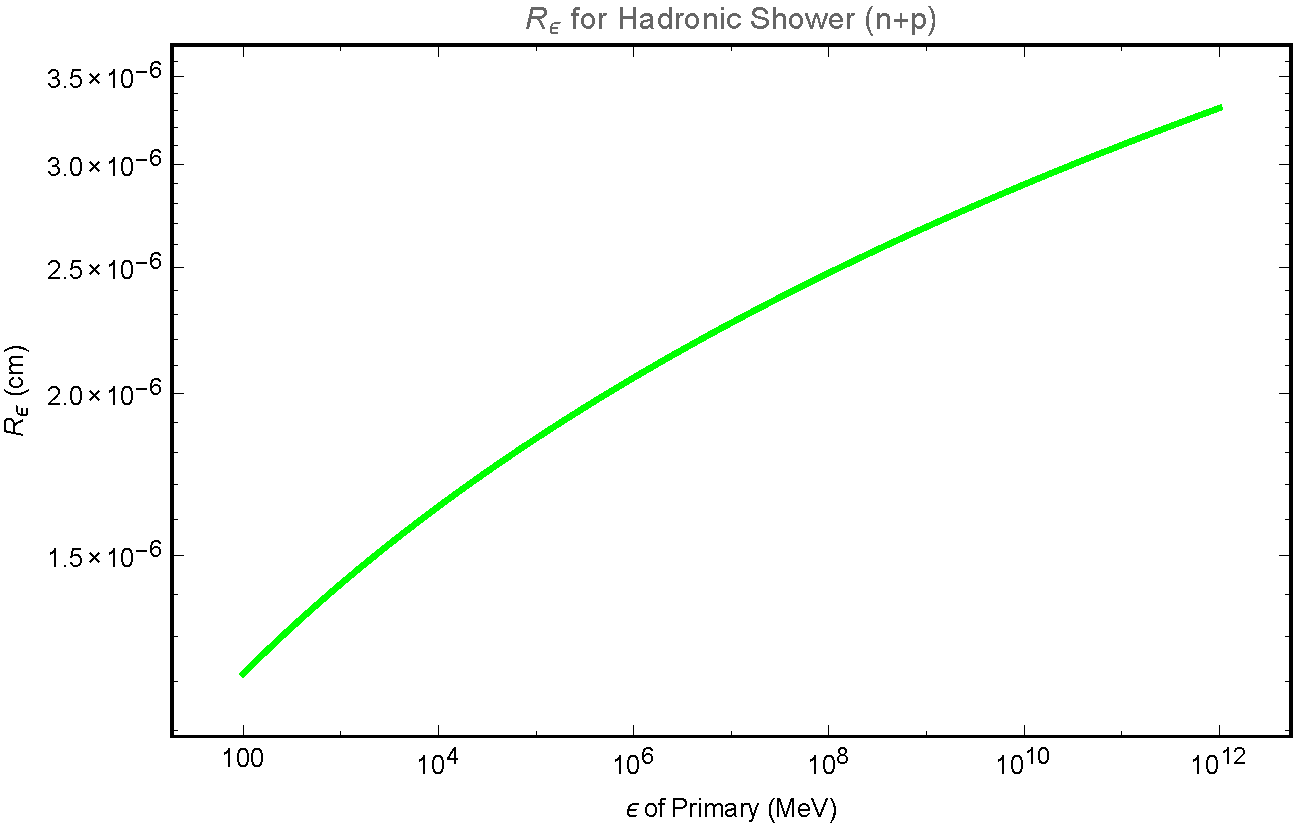
\includegraphics[scale=.35]{hadronic.pdf}
\end{figure}

\section{Example: Q Ball Dark Matter}
In various supersymmetric extensions of the standard model (SM), non-topological solitons called Q balls can be produced in the early universe \cite{Coleman:1985ki, Kusenko:1997si}. If these Q balls were stable, they would comprise a component of the dark matter today. Q balls can be classified into two groups: supersymmetric electrically charged solitons (SECS) and supersymmetric electrically neutral solitons (SENS). When a neutral baryonic Q ball interacts with a nucleon, it absorbs its baryonic charge as a minimum-energy configuration and induces the dissociation of the nucleon into free quarks. In this process (known as the ``KKST" process), $\sim \text{GeV}$ of energy is released through the emission of 2-3 pions \cite{Dine:2003ax}. The KKST process provides a useful way to detect such Q balls. The cross section for interaction is approximately the geometric cross section
\begin{equation}
\sigma_Q \simeq \pi R_Q^2.
\end{equation}
In gauge-mediated models with flat scalar potentials, the Q ball mass and radius are given by
\begin{equation}
M_Q \sim m_F Q^{3/4}, ~~~ R_Q \sim m_F^{-1} Q^{1/4},
\end{equation}
where $m_F$ is related to the scale of supersymmetry breaking (messenger scale). The condition $M_Q/Q < m_p$ ensures that the Q ball is stable against decay to nucleons \cite{Dine:2003ax}.

Note that a sufficiently massive Q ball will become a black hole if the Q ball radius is less than the Schwarzschild radius $R_Q \lesssim R_s \sim G M_Q$. In the model described above, this translates into the condition
\begin{equation}
m_F \l\frac{\Mpl}{m_F}\r^3 \lesssim m_Q, ~~~ \l\frac{\Mpl}{m_F}\r^4 \lesssim Q.
\end{equation}
For Q ball masses of this order, gravitational interactions become relevant while the KKST interaction ceases to exist.

\subsection{Q ball Explosiveness}
We assume that for each Q ball collision, there is equal probability to produce $\pi^0, \pi^+$ and $\pi^-$ under the constraint of charge conservation. In the notation of Section \textcolor{blue}{overview}, $n_{\pi} \sim \OO(10)$ pions are released with $\epsilon_{\pi} \sim \text{GeV}$. \textcolor{blue}{The mean distance travelled by a relativistic particle before decaying is $d = \gamma v \tau$. $\gamma \approx 5$, so for neutral pions $d_{\pi^0} \sim 10^{-5} ~\text{cm}$ while for charged pions, $d_{\pi^\pm} \sim 10 ~\text{m}$.}

Numerous experiments have studied the effects of $50 - 500 ~\text{MeV}$ pions incident upon complex nuclei targets such as carbon. It is found that there is roughly equal cross section of order $\sim 0.1 ~\text{barn}$ for a (neutral or charged) pion to either scatter elastically, scatter inelastically, or become absorbed with no final state pion \cite{Pionnuclear}. Of these possibilities, pion absorption is the most relevant for energy loss as this will induce a hadronic shower. During this process, $\sim$ 2-3 hadrons (i.e. protons, neutrons, alpha particles) are emitted. \textcolor{blue}{Point of this paragraph: argue that KKST range lies within trigger size}

Therefore, Q balls with sufficiently large cross-section $\sigma_Q \gtrsim 10^{-4} \lambda_T^2$ will result in explosions. This is plotted in Figure \textcolor{blue}{figure}. For the model described in Section \textcolor{blue}{previous section}, the Q ball cross section is related to its mass $m_Q = \sigma_Q^{3/2} m_F^4$ and $Q = \sigma_Q^2 m_F^4$. Therefore, find that
\begin{equation}
m_Q \gtrsim 10^8 ~\text{g} \l\frac{m_F}{\text{TeV}}\r^4, ~~~~ Q \gtrsim 10^{38} \l\frac{m_F}{\text{TeV}}\r^4
\end{equation}
is capable of triggering runaway fusion in a heavy $\sim 1.25 M_{\odot}$ WD for which $\lambda_T \sim 10^5 ~\text{cm}$.

\begin{figure}
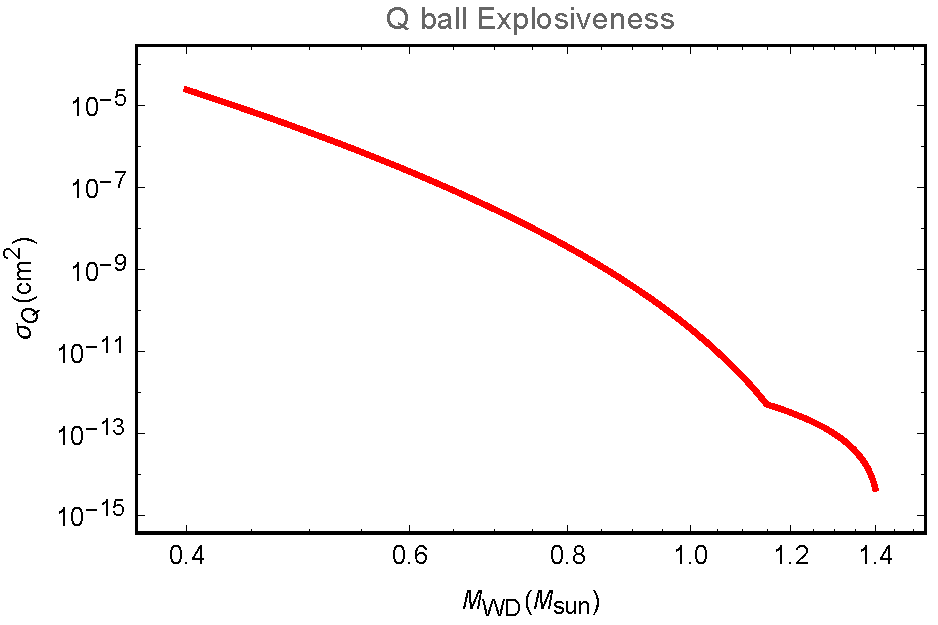
\includegraphics[scale=.45]{boomQball.pdf}
\end{figure}


\subsection{Q ball Constraints}
The transit rate for an ultra-heavy DM state through a WD is given by
\begin{equation}
\Gamma_\text{DM} = n_Q \sigma_g v \sim \frac{\rho_{\text{DM}}}{m_\text{DM}} \pi R_{s}^2 \l\frac{v_\text{esc}^2}{v}\r,
\end{equation}
where $v \sim 10^{-3}$ is the virial velocity of DM and $\rho_{\text{DM}}$ is the energy density of DM in the region of interest. $\sigma_g$ denotes the capture cross-section including the gravitational Sommerfeld enhancement.


The existence of heavy white dwarfs can rule out Q ball DM. Considering a $1.25 M_{\odot}$ WD in the local dark matter halo $\rho_{\text{DM}} \sim 0.3 ~\text{GeV}/\text{cm}^3$, we find that a Q ball of mass $m_Q \lesssim 10^{20} ~\text{g}$ will transit with a rate $\Gamma_Q \gtrsim \text{Gyr}^{-1}$. If we instead consider (recently discovered) heavy white dwarfs in the galactic center $\rho_{\text{DM}} \sim 10^3 ~\text{GeV}/\text{cm}^3$, Q balls of mass $m_Q \lesssim 10^{24} ~\text{g}$ will transit within a Gyr.

\section{Discussion}

\appendix

\section{Detail Study of Heating Lengths}
\label{app:heatinglengthfull}

\section{Acknowledgements}
We would like to thank S. Rajendran, K. Harigaya, R. McGehee, and J. Wurtele for many stimulating discussions. 

\bibliography{Qballs}

\end{document}
